\documentclass[pdflatex,ja=standard,fleqn]{bxjsarticle}
\usepackage{ascmac,amsmath,amssymb,type1cm, tikz, graphicx}

\title{材料の変形と破壊レポート}
\author{J4-210447 川村朋広}
\begin{document}
\maketitle


\section*{1}
\begin{figure}[htbp]
    \centering
    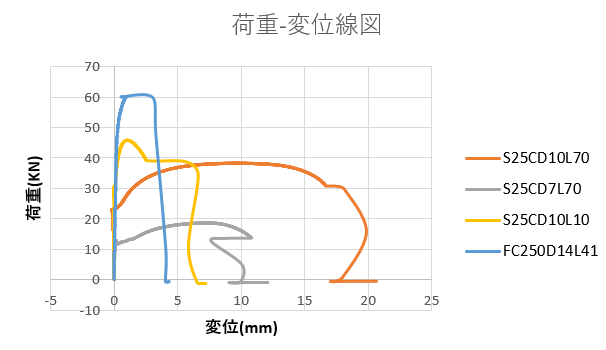
\includegraphics[width=10cm]{henikajyu.png}
\end{figure}
\begin{figure}[htbp]
    \centering
    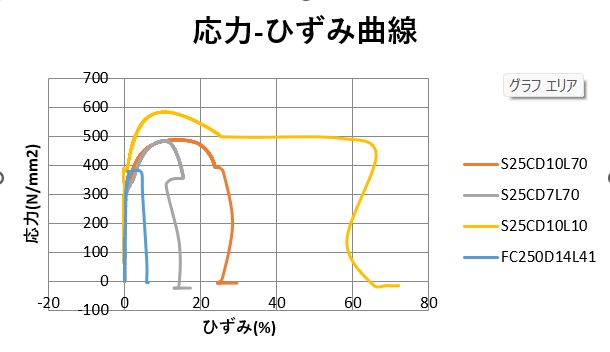
\includegraphics[width=10cm]{oryokuhizumi.png}
\end{figure}
\section*{2}
長さが同じ場合について、断面積が大きいほど最大荷重が大きくなるが、最大応力はほぼ等しい。ひずみは断面積が大きい方が大きい。\\
一方、断面積が同じ場合について考えると、$L=70$の場合$L=10$の場合よりも最大荷重時のひずみが大きくなることがわかる。
また、軟鋼は鋳鉄よりも最大応力が大きい傾向にあるといえる。
\section*{3}
\begin{figure}[htbp]
    \centering
    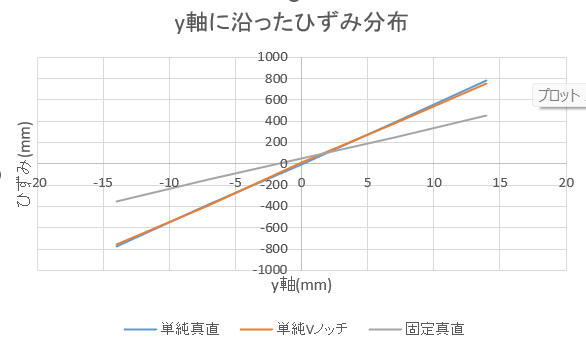
\includegraphics[width=10cm]{hizumi2.png}
\end{figure}
\begin{figure}[htbp]
    \centering
    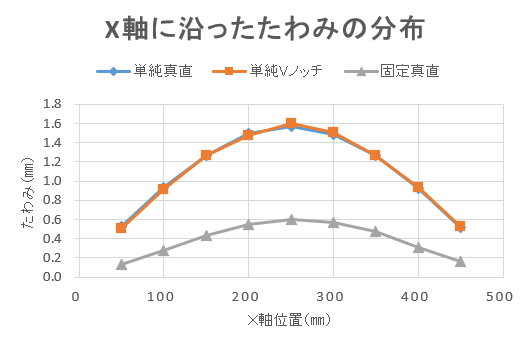
\includegraphics[width=10cm]{tawami7.png}
\end{figure}
\section*{4}
梁の中央に集中荷重$P=10000N$をかけるとする。\\
梁の長さ$l=0.5$\\
ヤング率$E=205×10^{9}$\\
梁の断面二次モーメント$I_{zz}=8.7×10^{-8}$\\
であるとする。\\
(a)単純支持の場合\\
両端の支持棒から受ける反力はともに$\frac{P}{2}$\\
$0<x<\frac{l}{2}$のとき\\
モーメントのつり合いから
\begin{eqnarray}
    M(x)=\frac{P}{2}x
\end{eqnarray}
より、
\begin{eqnarray}
    \theta_{1}&=&\frac{dv_{1}}{dx}\\
    &=&\int -\frac{M(x)}{EI_{zz}}dx\\
    &=&-\frac{P}{4EI_{zz}}x^{2}+C_{1}
\end{eqnarray}
$\frac{l}{2}<x<l$のとき
\begin{eqnarray}
    M(x)=-\frac{P}{2}x+\frac{P}{2}l
\end{eqnarray}
より、
\begin{eqnarray}
    \theta_{2}&=&\frac{dv_{2}}{dx}\\
    &=&\int -\frac{M(x)}{EI_{zz}}dx\\
    &=&\frac{P}{4EI_{zz}}(l-x)^{2}+C_{2}
\end{eqnarray}
境界条件
\begin{align}
    &v_{1}(0)=v_{2}(l)=0\\
    &v_1\left(\frac{l}{2}\right)=v_{2}\left(\frac{l}{2}\right)\\
    &\theta_{1}\left(\frac{l}{2}\right)=\theta_{2}\left(\frac{l}{2}\right)
\end{align}
より、
\begin{align}
    &v_{1}(x)=-\frac{P}{EI_{zz}}\left(\frac{1}{12}x^{3}-\frac{1}{16}l^{2}x\right)\\
    &v_{2}(x)=-\frac{P}{EI_{zz}}\left[-\frac{1}{12}(l-x)^{3}-\frac{1}{16}l^{2}x+\frac{1}{16}l^{3}\right]
\end{align}
断面の位置を$x=2.0×10^{-1}<\frac{l}{2}$と置くと、曲げげモーメント$M_{zx}$は
\begin{eqnarray}
    M_{zx}=-\frac{P}{2}x
\end{eqnarray}
とあらわせるから、ひずみ$\epsilon_{xx}$は
\begin{eqnarray}
    \epsilon_{xx}=-\frac{M_{zx}}{EI_{zz}}y=5.6×10^{-2}y
\end{eqnarray}
とあらわされる。\\
(b)固定支持の場合\\
両端から受ける反力はともに$\frac{P}{2}$\\
また、両端にかかる曲げモーメントの大きさは等しいのでそれぞれ$M^{\prime}$とおく\\
$0<x<\frac{l}{2}$のとき\\
モーメントのつり合いから
\begin{eqnarray}
    M(x)=\frac{P}{2}x+M^{\prime}
\end{eqnarray}
より、
\begin{eqnarray}
    \theta_{1}&=&\frac{dv_{1}}{dx}\\
    &=&\int -\frac{M(x)}{EI_{zz}}dx\\
    &=&-\frac{1}{EI_{zz}}\left(\frac{P}{4}x^{2}+M^{\prime}x+C_{1}\right)
\end{eqnarray}
$\frac{l}{2}<x<l$のとき
\begin{eqnarray}
    M(x)=-\frac{P}{2}x+\frac{P}{2}l+M^{\prime}
\end{eqnarray}
より、
\begin{eqnarray}
    \theta_{2}&=&\frac{dv_{2}}{dx}\\
    &=&\int -\frac{M(x)}{EI_{zz}}dx\\
    &=&\frac{1}{4EI_{zz}}\left[\frac{P}{4}(l-x)^{2}+M^{\prime}x+C_{2}\right]
\end{eqnarray}
境界条件
\begin{align}
    &v_{1}(0)=v_{2}(l)=0\\
    &\theta_{1}(0)=\theta_{2}(1)=0\\
    &v_{1}\left(\frac{l}{2}\right)=v_{2}\left(\frac{l}{2}\right)\\
    &\theta_{1}\left(\frac{l}{2}\right)=\theta_{2}\left(\frac{l}{2}\right)
\end{align}
より、
\begin{align}
    &v_{1}(x)=-\frac{P}{EI_{zz}}\left(\frac{1}{12}x^{3}-\frac{1}{16}lx^{2}\right)\\
    &v_{2}(x)=-\frac{P}{EI_{zz}}\left[\frac{1}{12}(l-x)^{3}-\frac{1}{16}lx^{2}+\frac{1}{8}l^{2}x-\frac{1}{16}l^{3}\right]
\end{align}
断面の位置を$x=2.0×10^{-1}<\frac{l}{2}$と置くと、曲げげモーメント$M_{zx}$は
\begin{eqnarray}
    M_{zx}=\frac{Pl}{8}-\frac{P}{2}x
\end{eqnarray}
とあらわせるから、ひずみ$\epsilon_{xx}$は
\begin{eqnarray}
    \epsilon_{xx}=-\frac{M_{zx}}{EI_{zz}}y=2.1×10^{-2}y
\end{eqnarray}
とあらわされる。
\section*{5}
梁の両端を単純支持する場合の負荷点のたわみの理論値は$1.5mm$で、実際の結果はおよそ$1.6mm$でそこまで誤差がなかった。一方で、梁の両端を固定した場合の理論値は$0.37mm$であるのに対し、実際の値はおよそ$0.6mm$と大きくずれる結果となった。\\
おおよそ棒の中央でたわみの最大値をとっていることより、このずれは両端の固定の度合いが甘くて、梁の曲げモーメントの大きさがおおきくなったのが原因だと考えられる。\\
ひずみついては理論値が$y=0$のとき$0$、$y=7$のとき$393$、$y=14$のとき$785$で実験値と理論値で大きな差がない。一方で両端を固定した場合は理論値が$y=0$のとき$0$、$y=7$のとき$147$、$y=14$のとき$294$で実際の値は理論値と大きくずれる結果となった。\\
$y=0$のときに$0$を取っていないのことより、計測する$y$座標のずれが原因であると考えられる。また、両端の固定が甘くモーメントの大きさが大きくなって直線の傾きが大きくなったのもずれの原因と考えられる。\\
\end{document}